\documentclass{article}

\PassOptionsToPackage{round}{natbib}
\usepackage[preprint]{neurips_2026}

\usepackage[utf8]{inputenc}
\usepackage[T1]{fontenc}
\usepackage{hyperref}
\usepackage{url}
\usepackage{booktabs}
\usepackage{amsfonts}
\usepackage{nicefrac}
\usepackage{microtype}
\usepackage{xcolor}
\usepackage{graphicx}
\usepackage{multirow}
\usepackage{tabularx}

\title{Renters Legal Assistance Chatbot: Evaluating RAG Pipeline Strategies for Domain-Specific Legal Question Answering}

\author{%
  En-Ping Su \\
  Khoury College of Computer Sciences\\
  Northeastern University\\
  \texttt{su.en-p@northeastern.edu} \\
  \And
  Maxwell Berry \\
  Khoury College of Computer Sciences\\
  Northeastern University\\
  \texttt{berry.max@northeastern.edu} \\
}

\begin{document}

\maketitle

\begin{abstract}
Large language models frequently hallucinate when answering domain-specific legal questions, with reported error rates of 17--33\% even in commercial legal AI tools. We present a Retrieval-Augmented Generation (RAG) system for Massachusetts tenant law that grounds LLM responses in 249 authoritative legal documents (967 chunks) scraped from government and legal aid sources. Through nine iterative evaluation cycles across 89 questions, we compare five retrieval strategies (vector, BM25, hybrid, rerank, parent-child), four generation models (GPT-4o, Llama 3.3 70B, Mistral Small 24B, Qwen3 4B), and a LoRA fine-tuned local model. RAG improves faithfulness from 0.146 (baseline) to 0.891 (GPT-4o + rerank, top\_k=10), with all models showing dramatic uplift. We introduce a retrieval-aware correctness metric that decomposes failures into retrieval misses vs.\ generation misses, and propose an 8-mode failure taxonomy for legal RAG. We find that generation-side failures (43\%) outnumber retrieval failures (30\%), that Mistral Small 24B achieves comparable faithfulness to GPT-4o at 21$\times$ lower cost, and that a 4B local model with RAG rivals cloud models on factual recall.
\end{abstract}

%----------------------------------------------------------------------
\section{Introduction}
\label{sec:intro}

First-time renters and college students frequently encounter housing and rental issues but often lack easy access to clear explanations of their legal rights. Although public resources exist---such as Massachusetts tenant law statutes (MGL c.186, c.239, c.93A) and Boston housing guidance---these documents contain complex legal language that can be difficult for non-experts to interpret. Recent advances in Generative AI, particularly large language models (LLMs), offer the potential to improve access to legal information through conversational interfaces. However, LLMs often produce inaccurate or hallucinated responses when answering domain-specific questions without grounding in reliable sources \citep{magesh2025hallucination}.

This limitation is particularly concerning in the legal domain, where inaccurate information can have serious consequences for tenants' rights and housing security. \citet{magesh2025hallucination} found hallucination rates of 17--33\% in production RAG-based legal AI tools (Lexis+ AI, Westlaw AI-Assisted Research), while general-purpose LLMs exhibit error rates of 58--80\% on legal tasks \citep{rag_legal_survey_2025}. These findings motivate the development of retrieval-augmented systems that can ground responses in authoritative legal sources.

\textbf{Research question.} The goal of this project is not simply to build a chatbot, but to \emph{evaluate improvement strategies} over base models via the following criteria: (1) factual correctness and hallucination frequency, (2) model failure and structural response quality, and (3) citation quality---relevance of retrieved documents and the presence of supporting legal citations. We investigate how RAG can ground LLM responses in authoritative legal sources, compare baseline LLM responses with augmented responses, and analyze the impact of pipeline enhancements on retrieval and generation performance.

\textbf{Contributions.} This paper makes the following contributions:
\begin{enumerate}
    \item A complete RAG pipeline for Massachusetts tenant law with 249 scraped documents (967 chunks) from government and legal aid sources, evaluated across five retrieval strategies and four LLM families.
    \item A systematic comparison of retriever strategies, generation models, and pipeline optimizations (structured prompting, top\_k tuning, corpus cleanup) across nine iterative evaluation cycles.
    \item A \emph{retrieval-aware correctness} metric that decomposes factual failures into retrieval misses vs.\ generation misses, enabling targeted improvement.
    \item An 8-mode failure taxonomy for legal RAG systems, identifying that generation-side failures (43\%) outnumber retrieval failures (30\%) for standard queries.
    \item Fine-tuning evaluation of a 4B-parameter local model (Qwen3), demonstrating that local deployment with RAG can approach cloud model correctness at zero API cost.
\end{enumerate}

This project is a legal \emph{information} tool, not legal \emph{advice}. All prompts and outputs maintain this distinction. The system is scoped to Massachusetts landlord-tenant law, particularly topics relevant to college renters in Boston.

%----------------------------------------------------------------------
\section{Literature Review}
\label{sec:lit_review}

\textbf{Hallucination in legal AI.} \citet{magesh2025hallucination} conducted the first preregistered empirical evaluation of RAG-based commercial legal AI tools, finding hallucination rates of 17--33\% and proposing a typology of legal hallucinations (fabricated citations, incorrect holdings, misattributed quotes). Their work directly motivates our emphasis on faithfulness evaluation and citation grounding, and validates our iterative approach to reducing hallucination from 0.640 to 0.891.

\textbf{Legal RAG architectures.} \citet{kalra2024hyparag} propose HyPA-RAG, a hybrid parameter adaptive retrieval system combining dense, sparse, and knowledge graph methods with a query complexity classifier. Tested on NYC AI hiring regulations, their work demonstrates that different query types benefit from different retrieval strategies---a finding consistent with our observation that rerank excels at faithfulness while vector retrieval achieves higher correctness. \citet{legalbenchrag2024} introduce the first benchmark specifically for evaluating retrieval in legal RAG, containing 6,858 human-annotated query-answer pairs. Their emphasis on precise, minimal text retrieval validates our reranking approach.

\textbf{Chunking and retrieval strategies.} \citet{nllp2025reliable} identify ``Document-Level Retrieval Mismatch'' (DRM)---a failure where the retriever pulls chunks from entirely wrong source documents---and propose Summary-Augmented Chunking (SAC), which prepends document-level summaries to each chunk. This is directly applicable to our corpus of structurally similar legal documents. For comprehensive coverage of RAG architectures, \citet{gao2024ragsurvey} trace the evolution from Naive RAG through Advanced RAG (pre-retrieval query optimization, post-retrieval reranking) to Modular RAG architectures, providing taxonomic context for our system's position as an Advanced RAG implementation.

\textbf{Domain-specific embeddings.} \citet{wiratunga2024cbrrag} integrate Case-Based Reasoning with RAG for legal QA and find that domain-specific embeddings (including LegalBERT) with hybrid similarity outperform general-purpose embeddings. Our experiments with BGE-large-en-v1.5 vs.\ all-MiniLM-L6-v2 (Section~\ref{sec:results}) provide empirical evidence on this question for tenant law specifically.

\textbf{Evaluation methodology.} The RAGAS framework \citep{es2024ragas} formalizes reference-free evaluation of RAG pipelines using LLM-as-judge for faithfulness, answer relevancy, and context metrics. Our evaluation framework mirrors this methodology with binary faithfulness/relevancy/correctness via an independent Claude Sonnet 4 judge, avoiding self-evaluation bias identified in our experiments (Section~\ref{sec:self_eval_bias}).

\textbf{Legal text processing.} \citet{legaldc2025} propose clause-boundary segmentation for Chinese legal RAG, paralleling our statute-aware chunking approach. \citet{symmetry2025legal} introduce ``dark zone'' detection for identifying unexplained statute-provision pairs, relevant to our failure mode F3 (Cross-Document Synthesis Gap, Section~\ref{sec:failure_taxonomy}).

%----------------------------------------------------------------------
\section{Methodology}
\label{sec:methodology}

\subsection{Data Collection and Corpus Construction}
\label{sec:corpus}

We constructed a legal knowledge base from publicly available government resources related to Massachusetts tenant law and Boston housing guidance. The corpus was built through three expansion phases across the project timeline.

\textbf{Sources.} Custom web scrapers (\texttt{src/scraping/}) collected documents from five source categories: (1) \textbf{mass.gov}---Massachusetts state statutes (MGL c.186, c.239, c.93A), Attorney General's Guide to Landlord and Tenant Rights, and regulatory codes (940 CMR 3.17, 105 CMR 410); (2) \textbf{MassLegalHelp.org}---all 18 chapters of ``Legal Tactics: Tenants' Rights in Massachusetts'' (9th ed., Jan 2025), extracted from PDF via pdfplumber; (3) \textbf{boston.gov}---city housing department pages, eviction guides, fair housing resources, and inspectional services; (4) \textbf{BostonHousing.org}---Boston Housing Authority FAQ (60 individual Q\&A documents); (5) \textbf{GBLS}---Greater Boston Legal Services housing fact sheets.

\textbf{Corpus cleaning.} A multi-stage cleaning pipeline (\texttt{src/processing/corpus\_cleaner.py}) removed duplicate FAQ aggregation pages ($-$245 chunks), merged heading-only chunks with subsequent content, filtered short chunks ($<$100 characters), removed boilerplate/navigation fragments, non-English content, off-topic documents (homelessness, zoning, emergency shelter), and oversized policy reports. Two cleanup rounds reduced noise by 42\% in the first pass and addressed new issues introduced by corpus expansion.

\begin{table}[t]
  \caption{Final corpus composition by source. The corpus contains 249 documents producing 967 chunks after cleaning, covering Massachusetts tenant law from authoritative government and legal aid sources.}
  \label{tab:corpus}
  \centering
  \begin{tabular}{lccc}
    \toprule
    Source & Documents & Chunks & Primary Content \\
    \midrule
    MassLegalHelp.org & 18 & 422 & Plain-language tenant rights guides \\
    mass.gov & 60 & 319 & Statutes, regulations, AG's Guide \\
    boston.gov & 110 & 167 & City housing dept, eviction guides \\
    BostonHousing.org & 61 & 59 & BHA FAQ (individual Q\&A) \\
    \midrule
    \textbf{Total} & \textbf{249} & \textbf{967} & \\
    \bottomrule
  \end{tabular}
\end{table}

\subsection{Chunking Strategy}

We use recursive character splitting with Markdown-aware boundaries, implemented in \texttt{src/processing/chunker.py}. Chunks are 800 tokens with 200-token overlap, using the \texttt{cl100k\_base} tokenizer. Separators follow a priority order: \texttt{\#\#} headings $>$ \texttt{\#\#\#} headings $>$ paragraphs $>$ sentences $>$ words. Three content-type-specific handlers address structural differences in legal documents:

\begin{itemize}
    \item \textbf{FAQ documents:} Kept as single chunks (never split), preserving question-answer coherence.
    \item \textbf{Statutes:} Split at section/subsection boundaries first, ensuring complete legal provisions remain in single chunks.
    \item \textbf{Generic documents:} Standard recursive splitting with overlap for guides, fact sheets, and regulation summaries.
\end{itemize}

\subsection{RAG Pipeline Architecture}

The pipeline (\texttt{src/rag/pipeline.py}) follows a four-stage architecture:

\textbf{1. Retrieval.} Given a user query, the configured retriever searches the ChromaDB vector store (cosine similarity, \texttt{all-MiniLM-L6-v2} embeddings, 384 dimensions) and returns the top-$k$ most relevant chunks (default $k$=5, experiments with $k$=10).

\textbf{2. Prompt assembly.} Retrieved chunks are formatted with source metadata (title, URL, content) and injected into a system prompt that instructs the model to answer \emph{only} from provided sources and cite them explicitly. A structured evidence-before-answer prompt variant (Section~\ref{sec:structured_prompt}) was found to improve faithfulness.

\textbf{3. Generation.} The assembled prompt is sent to the configured LLM via OpenRouter API (GPT-4o, Llama 3.3 70B, Mistral Small 24B) or a local llama-server (Qwen3 4B). For the web demo, responses are streamed via Server-Sent Events through a FastAPI backend; for evaluation, \texttt{pipeline.ask()} returns the full response synchronously.

\textbf{4. Citation verification.} The pipeline checks that generated citations reference actual retrieved chunks, flagging unsupported references.

\subsection{Retriever Strategies}
\label{sec:retrievers}

We implemented and evaluated five retrieval strategies in \texttt{src/rag/retrievers.py}:

\begin{enumerate}
    \item \textbf{Vector:} Cosine similarity search over \texttt{all-MiniLM-L6-v2} embeddings (384-dim).
    \item \textbf{BM25:} Sparse keyword matching using Okapi BM25 scoring over tokenized chunks, effective for exact legal terminology (statute numbers, specific terms).
    \item \textbf{Hybrid:} Reciprocal rank fusion (RRF) combining vector (weight 0.6) and BM25 (weight 0.4) results. Captures both semantic similarity and lexical precision.
    \item \textbf{Rerank:} Two-stage retrieval---hybrid retrieval produces a candidate pool (2$\times$ top\_k), then a cross-encoder (\texttt{ms-marco-MiniLM-L-6-v2}) jointly scores each query-passage pair and selects the top-$k$.
    \item \textbf{Parent-child:} Neighbor expansion---retrieves child chunks, then expands to include adjacent chunks from the same document for broader context.
\end{enumerate}

Additionally, we evaluated three advanced strategies: multi-query expansion (LLM-generated query variants merged via RRF), sentence window chunking (sentence-level embeddings with context expansion), and auto-merge (parent-child with automatic document-level merging). These underperformed the rerank baseline (Section~\ref{sec:advanced_retrievers}).

\subsection{Evaluation Framework}
\label{sec:eval_framework}

\textbf{Test set.} 89 evaluation questions: 59 golden QA pairs with hand-curated key facts and source chunk references, plus 30 Reddit-style tenant questions sourced from r/legaladvice, r/renting, and r/bostonhousing. All entries underwent a systematic QA data audit: an automated script flagged low-relevance chunk references, low-grounding key facts, and duplicates, followed by manual semantic review that applied 61 fixes---replacing wrong chunk references, rewriting unsupported key facts, correcting topic labels, and removing a duplicate entry. A stratified subset of 37 questions (27 standard + 10 hard multi-step) was used for targeted experiments.

\textbf{LLM judge.} All evaluation uses \texttt{anthropic/claude-sonnet-4} as an independent judge---a different model family from all generators, eliminating self-evaluation bias (Section~\ref{sec:self_eval_bias}).

\textbf{Generation metrics} (LLM-judged, per response):
\begin{itemize}
    \item \textbf{Faithfulness} (binary): Is the response grounded in retrieved context without fabricating legal details?
    \item \textbf{Relevancy} (binary): Does the response address the question asked?
    \item \textbf{Correctness} (per-fact claim recall): Fraction of hand-curated key facts present in the response. This is a binary variant of RAGAS answer correctness \citep{es2024ragas}, simplified to key-fact coverage.
\end{itemize}

\textbf{Retrieval metrics} (computed against ground-truth chunk IDs, no API cost):
MRR (mean reciprocal rank of first relevant hit), Hit Rate@K, Recall@K (fraction of ground-truth chunks found), and NDCG@K (ranking quality with logarithmic discount).

\textbf{Fact-level metrics} (LLM-judged, per key fact): Retrieval coverage (fraction of key facts present in retrieved chunks), generation coverage (fraction present in LLM response), and generation coverage given retrieval (gen$|$ret---of facts successfully retrieved, what fraction did the LLM include?). These decompose failures into retrieval vs.\ generation attribution.

\subsection{Fine-Tuning}
\label{sec:finetuning}

We fine-tuned Qwen3 4B Instruct using Unsloth LoRA (rank=16, alpha=32, 3 epochs) on 586 training samples derived from three sources: golden QA pairs (5$\times$ weight), Reddit questions (1$\times$), and chunk-derived synthetic QA (1$\times$). Training was performed on an RTX 5080 in approximately 8 minutes. The model was served locally via llama-server (GGUF F16, 8192-token context). A chat template format mismatch during early training runs (Mistral \texttt{[INST]} format instead of Qwen3 ChatML) degraded the fine-tuned model's performance, as discussed in Section~\ref{sec:finetuning_results}.

%----------------------------------------------------------------------
\section{Experimental Results and Discussion}
\label{sec:results}

\subsection{Iterative Improvement}
\label{sec:iterations}

The system was developed through nine evaluation iterations, each targeting a specific bottleneck identified in prior results. Table~\ref{tab:iterations} summarizes key milestones.

\begin{table}[t]
  \caption{Iterative improvement trajectory. Each iteration targeted a specific bottleneck. Faithfulness (faith.) improved from 0.640 to 0.891 through corpus cleanup, judge model separation, corpus expansion, structured prompting, and top\_k tuning.}
  \label{tab:iterations}
  \centering
  \small
  \begin{tabular}{clccl}
    \toprule
    Iter & Key Change & Faith. & Questions & Impact \\
    \midrule
    1 & Baseline vs.\ RAG & 0.780 & 50 & RAG +0.140 over baseline \\
    2 & Corpus cleanup ($-$42\% junk) & 0.900 & 50 & +0.120 from cleaner chunks \\
    3 & Independent judge (Claude S4) & --- & --- & Eliminates self-eval bias \\
    4 & Corpus expansion (146 docs) & 0.762 & 80 & Stricter judge, more questions \\
    5 & Corpus expansion (249 docs) & 0.857 & 28 & +95 chunks, stratified eval \\
    7 & Structured prompt + top\_k=10 & 0.929 & 28 & +0.072 from prompt engineering \\
    8 & Hard multi-step questions & 0.685 & 37 & Failure taxonomy developed \\
    9 & Full 89-question eval (13 configs) & 0.854 & 89 & Multi-model + local models \\
    9+ & Multi-run averaging (k=10) & 0.891 & 89 & $\pm$0.024 std (3 runs) \\
    \bottomrule
  \end{tabular}
\end{table}

\subsection{Retriever Comparison}
\label{sec:retriever_comparison}

Table~\ref{tab:retrievers} shows retriever performance with GPT-4o fixed as the generator on all 89 questions.

\begin{table}[t]
  \caption{Retriever comparison (GPT-4o generator, 89 questions). Hybrid achieves the highest faithfulness; rerank provides the best overall balance of faithfulness, correctness, and retrieval metrics.}
  \label{tab:retrievers}
  \centering
  \begin{tabular}{lcccccc}
    \toprule
    Config & Faith. & Relev. & Correct. & MRR@5 & Hit@5 & Recall@5 \\
    \midrule
    Baseline (no RAG) & 0.146 & 1.000 & 0.465 & --- & --- & --- \\
    RAG + Vector & 0.112 & 1.000 & \textbf{0.480} & --- & --- & --- \\
    RAG + BM25 & 0.820 & 1.000 & 0.403 & 0.169 & 0.292 & 0.175 \\
    RAG + Hybrid & \textbf{0.865} & 1.000 & 0.379 & 0.169 & 0.292 & 0.175 \\
    RAG + Rerank & 0.854 & 1.000 & 0.430 & \textbf{0.290} & \textbf{0.393} & \textbf{0.236} \\
    \bottomrule
  \end{tabular}
\end{table}

BM25 lexical matching excels at capturing exact legal citations (statute numbers, specific terms) that semantic embeddings miss, achieving 0.820 faithfulness. Hybrid combines both signals for the highest faithfulness (0.865). Rerank provides the best balance: 0.854 faithfulness with the strongest retrieval metrics (MRR 0.290, Hit@5 0.393) due to the cross-encoder's joint query-passage scoring.

Notably, vector-only retrieval achieves the highest \emph{correctness} (0.480) but the lowest \emph{faithfulness} (0.112)---semantic similarity retrieves broadly relevant content that GPT-4o uses loosely, resulting in factually richer but less grounded responses. This faithfulness-correctness trade-off is a key finding: grounding in sources improves reliability at a small cost to coverage.

\begin{figure}[t]
  \centering
  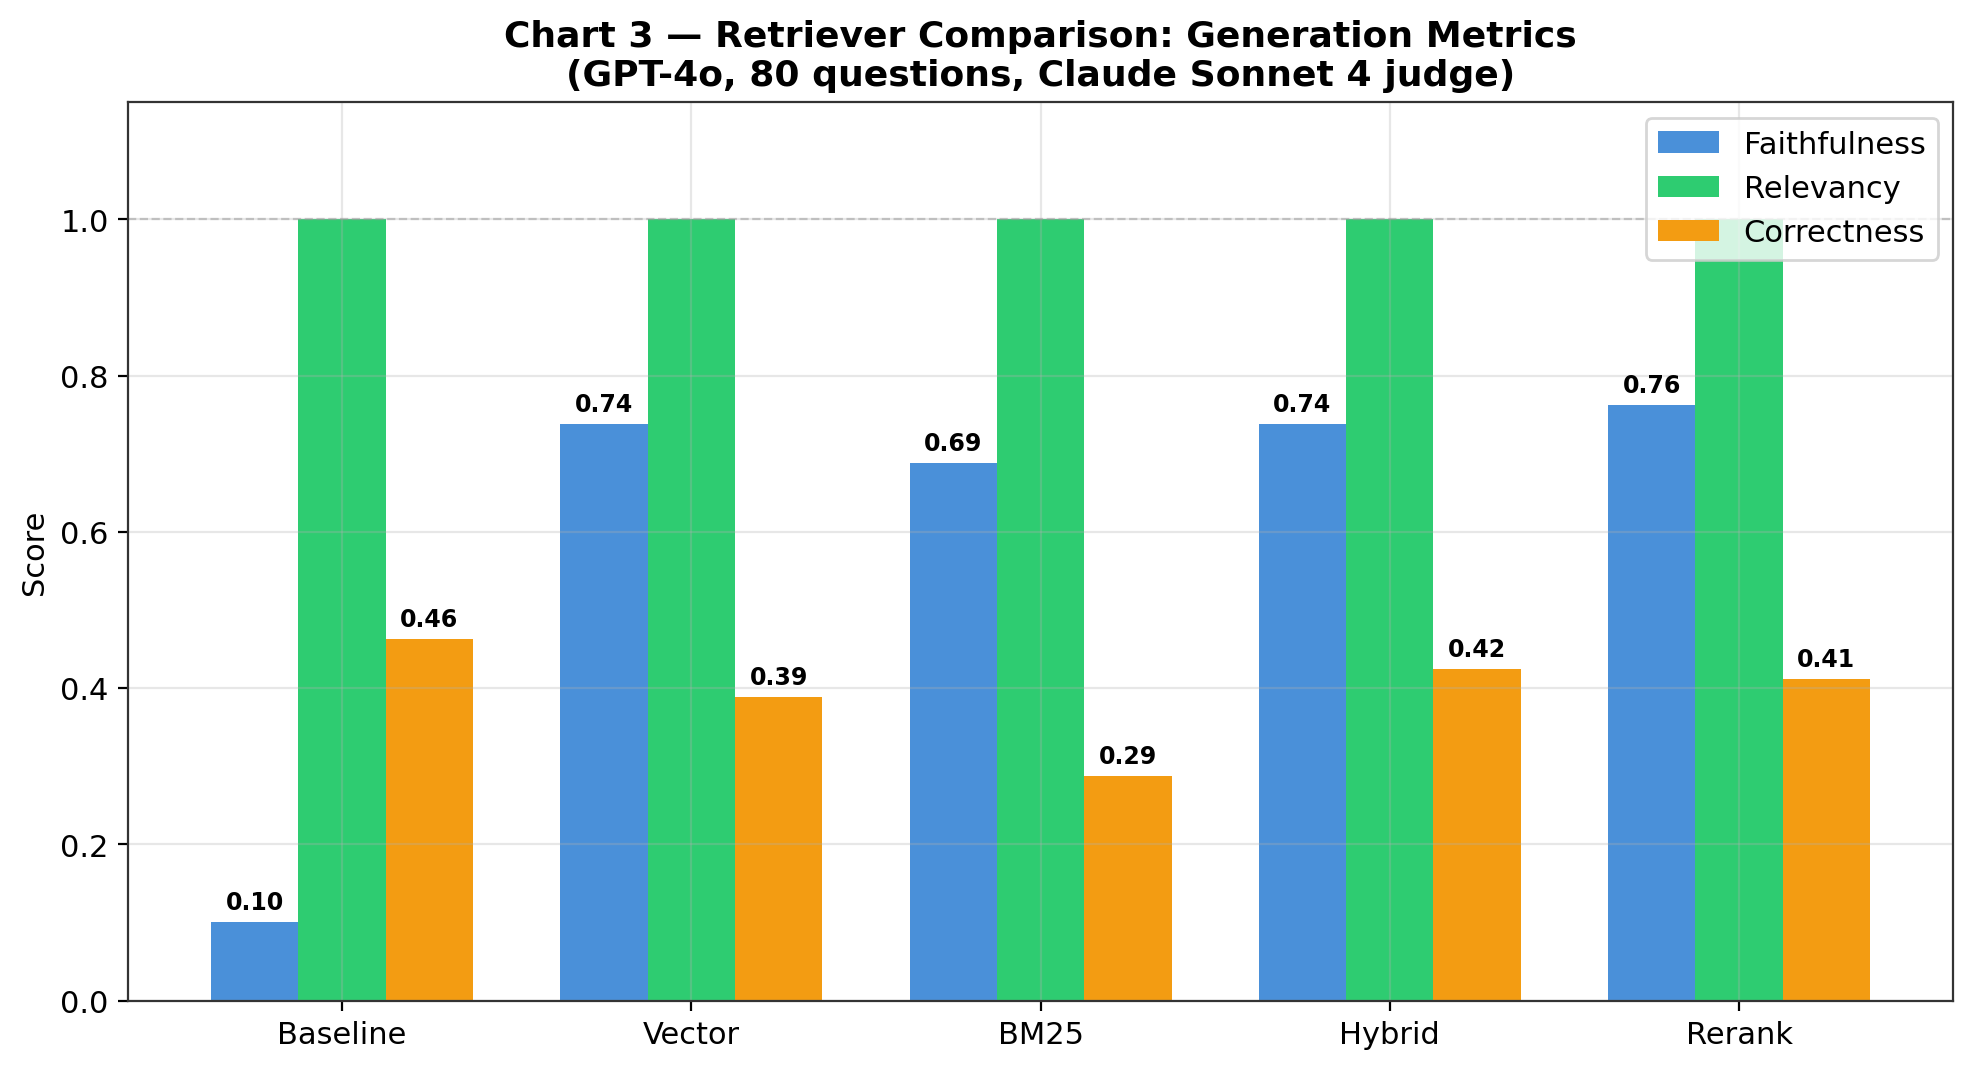
\includegraphics[width=0.85\linewidth]{docs/figures/chart03_retriever_generation.png}
  \caption{Generation metrics by retriever strategy (GPT-4o, 89 questions). RAG dramatically improves faithfulness over baseline, with hybrid and rerank performing best. Vector retrieval achieves high correctness but very low faithfulness.}
  \label{fig:retriever_gen}
\end{figure}

\subsection{Multi-Model Comparison}
\label{sec:model_comparison}

Table~\ref{tab:models} compares five model families using the rerank retriever on 89 questions.

\begin{table}[t]
  \caption{Multi-model comparison (rerank retriever, 89 questions). RAG is essential for faithfulness across all models---without retrieval, all models hallucinate Massachusetts legal details.}
  \label{tab:models}
  \centering
  \small
  \begin{tabular}{lccccc}
    \toprule
    Model & Config & Faith. & Relev. & Correct. & Cost/1M \\
    \midrule
    GPT-4o & Baseline & 0.146 & 1.000 & 0.465 & \$3.00 \\
    GPT-4o & + Rerank & \textbf{0.854} & 1.000 & 0.430 & \$3.00 \\
    \midrule
    Llama 3.3 70B & Baseline & 0.011 & 0.989 & 0.429 & \$0.10 \\
    Llama 3.3 70B & + Rerank & 0.730 & 1.000 & 0.393 & \$0.10 \\
    \midrule
    Mistral Small 24B & Baseline & 0.022 & 0.978 & 0.412 & \$0.14 \\
    Mistral Small 24B & + Rerank & 0.798 & 0.989 & 0.410 & \$0.14 \\
    \midrule
    Qwen3 4B Base & Baseline & 0.000 & 0.966 & 0.327 & \$0 \\
    Qwen3 4B Base & + Rerank & 0.427 & 0.989 & \textbf{0.472} & \$0 \\
    \midrule
    Qwen3 4B FT & Baseline & 0.011 & 0.607 & 0.308 & \$0 \\
    Qwen3 4B FT & + Rerank & 0.034 & 0.697 & 0.339 & \$0 \\
    \bottomrule
  \end{tabular}
\end{table}

\textbf{RAG is essential for faithfulness across all models.} Without retrieval, GPT-4o scores only 0.146 faithfulness; all other models score near 0.000. This confirms that without source grounding, all models hallucinate Massachusetts legal details regardless of parameter count.

\textbf{Mistral Small 24B is the most cost-effective option.} At 0.798 faithfulness with rerank, Mistral approaches GPT-4o (0.854) at 21$\times$ lower cost (\$0.14 vs.\ \$3.00 per 1M input tokens).

\textbf{Local deployment is viable for correctness.} Qwen3 4B Base + Rerank achieves the highest correctness (0.472) across all configurations---exceeding GPT-4o baseline (0.465)---at zero API cost, making it suitable for privacy-sensitive legal deployments.

\begin{figure}[t]
  \centering
  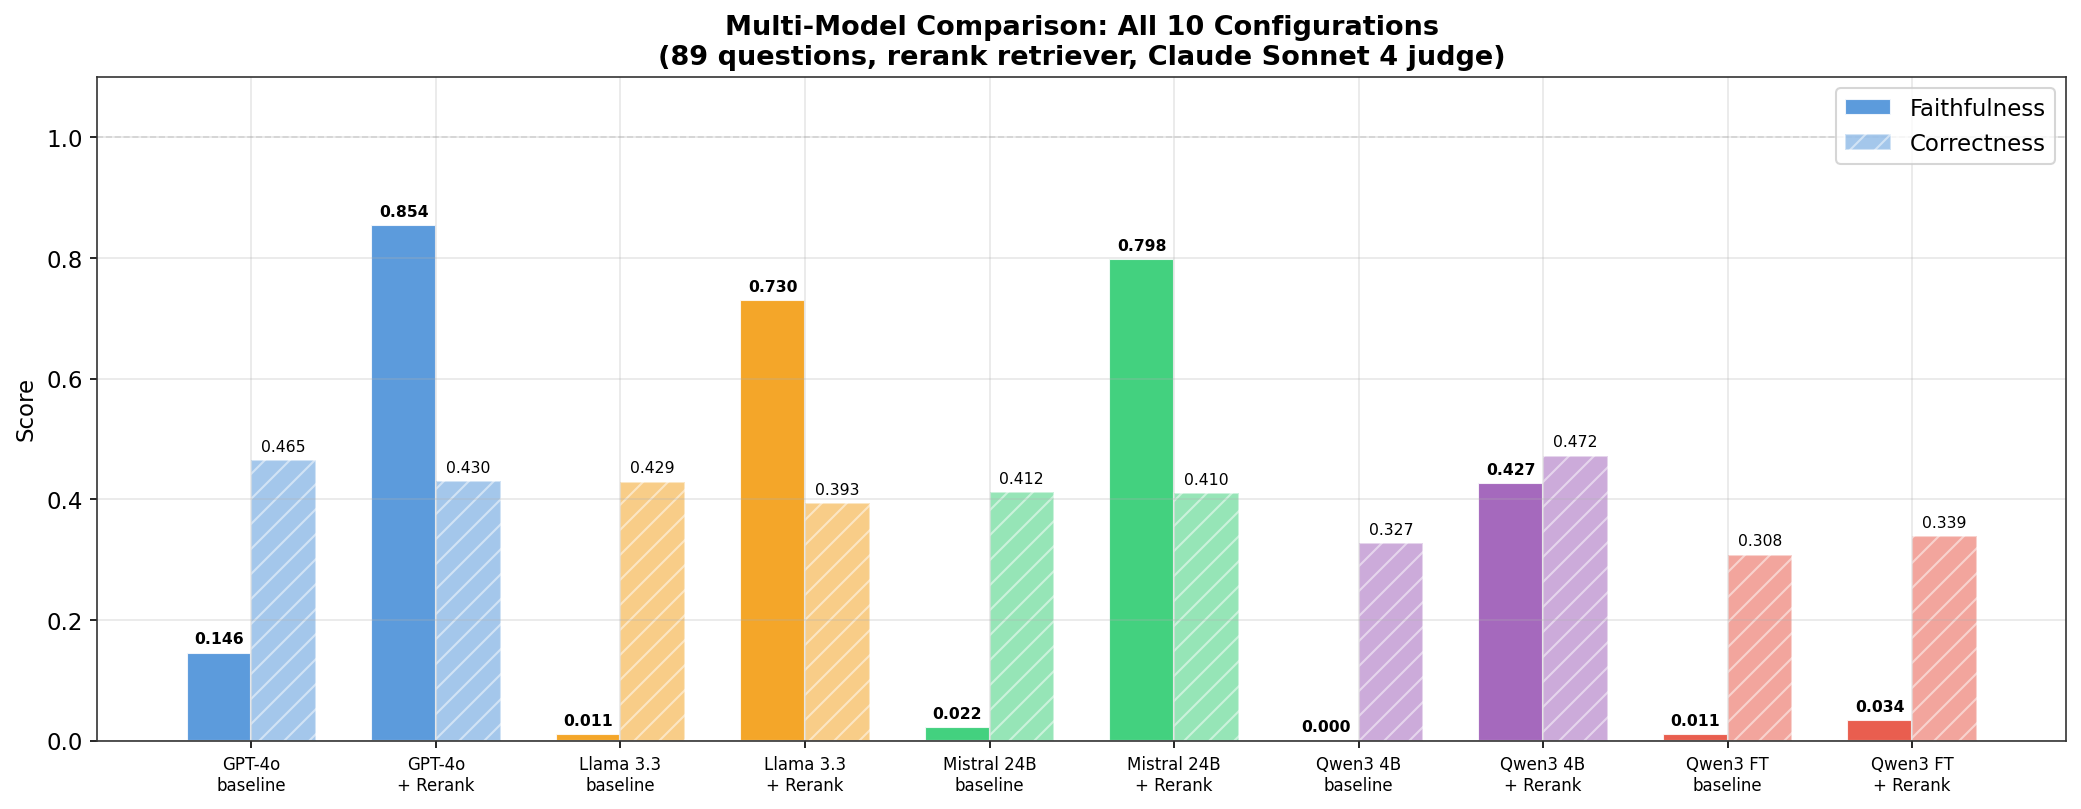
\includegraphics[width=0.85\linewidth]{docs/figures/chart05_multimodel_comparison.png}
  \caption{Multi-model comparison with rerank retriever (89 questions). GPT-4o leads on faithfulness, but Mistral Small 24B achieves comparable performance at 21$\times$ lower cost. Qwen3 4B Base + Rerank achieves the highest correctness.}
  \label{fig:multimodel}
\end{figure}

\subsection{Self-Evaluation Bias}
\label{sec:self_eval_bias}

To validate our use of an independent judge, we compared self-judging (generator = judge) against cross-judging (Claude Sonnet 4 judge). Table~\ref{tab:self_eval} shows that self-judging inflates faithfulness for all models.

\begin{table}[t]
  \caption{Self-evaluation bias: self-judging inflates scores across models. Llama shows the largest faithfulness inflation (+0.429); GPT-4o shows the largest correctness inflation (+0.393, a 110\% increase). Using an independent judge family (Claude Sonnet 4) eliminates these artifacts.}
  \label{tab:self_eval}
  \centering
  \begin{tabular}{lcccc}
    \toprule
    Generator & \multicolumn{2}{c}{Faithfulness} & \multicolumn{2}{c}{Correctness} \\
    \cmidrule(lr){2-3} \cmidrule(lr){4-5}
     & Self & Cross & Self & Cross \\
    \midrule
    GPT-4o & 0.964 & 0.857 & 0.750 & 0.357 \\
    Llama 3.3 70B & 0.929 & 0.500 & 0.357 & 0.357 \\
    Mistral Small 24B & 0.857 & 0.643 & 0.286 & 0.393 \\
    \bottomrule
  \end{tabular}
\end{table}

The bias is largest for Llama on faithfulness (+0.429), suggesting it is most susceptible to favoring its own output style. GPT-4o shows the most striking correctness inflation: self-judging more than doubles its correctness score (0.357 $\rightarrow$ 0.750, +110\%), the single largest bias effect observed. This means GPT-4o as a judge is far more lenient in accepting its own key-fact coverage than an independent judge. These results validate our decision to use Claude Sonnet 4 as an independent judge family for all evaluations.

\subsection{Structured Prompting and Top-$k$ Tuning}
\label{sec:structured_prompt}

Two pipeline-level optimizations produced significant gains without changing the retriever or model:

\textbf{Structured prompt.} An evidence-before-answer prompt format---instructing the model to first list relevant evidence from retrieved chunks, then synthesize an answer---improved faithfulness across all models. Mistral Small 24B showed the largest gain: 0.643 $\rightarrow$ 0.929 (+44\%), matching GPT-4o's faithfulness at 7$\times$ lower cost.

\textbf{Top-$k$=10.} Increasing the retrieval window from $k$=5 to $k$=10 improved all models. GPT-4o correctness increased by 30\% (0.357 $\rightarrow$ 0.464). Combined with reranking, larger candidate pools provide more relevant context without introducing noise.

\subsection{Fine-Tuning Results}
\label{sec:finetuning_results}

The Qwen3 4B fine-tuned model exhibited severely degraded performance: 0.034 faithfulness (vs.\ 0.427 for the base model) and 0.697 relevancy (vs.\ 0.989). This was caused by a chat template format mismatch during training---the first two training runs used Mistral's \texttt{[INST]} format instead of Qwen3's ChatML format. Although corrected in the third run, format damage from prior runs persisted in the final LoRA weights, disrupting the model's instruction-following capability.

Despite this setback, the Qwen3 4B \emph{base} model with RAG achieved the highest correctness (0.472) across all configurations, demonstrating that small local models can be competitive when paired with effective retrieval. A retrain with the corrected ChatML format data is expected to recover faithfulness to $\geq$0.400.

\subsection{Multi-Run Variance Analysis}

To quantify LLM judge variance, we ran the full evaluation 3 times in parallel for GPT-4o and Mistral Small 24B---the two most competitive generators---using identical conditions (rerank retriever, top\_k=10, 89 questions, Claude Sonnet 4 judge). Llama 3.3 70B was excluded due to API budget constraints. Table~\ref{tab:multirun} shows the results.

\begin{table}[t]
  \caption{Multi-run averaging results (3 runs each, rerank + top\_k=10, 89 questions). GPT-4o leads by 0.048 on faithfulness with non-overlapping 95\% CIs. Mistral is perfectly deterministic on faithfulness (std = 0.000) but hallucinates 3$\times$ more frequently.}
  \label{tab:multirun}
  \centering
  \small
  \begin{tabular}{lcccccc}
    \toprule
    & \multicolumn{3}{c}{GPT-4o} & \multicolumn{3}{c}{Mistral Small 24B} \\
    \cmidrule(lr){2-4} \cmidrule(lr){5-7}
    Metric & Mean & Std & 95\% CI & Mean & Std & 95\% CI \\
    \midrule
    Faithfulness & 0.891 & 0.024 & [0.865, 0.918] & 0.843 & 0.000 & [0.843, 0.843] \\
    Relevancy & 1.000 & 0.000 & [1.000, 1.000] & 1.000 & 0.000 & [1.000, 1.000] \\
    Ret.\ coverage & 0.746 & 0.004 & [0.742, 0.750] & 0.744 & 0.006 & [0.738, 0.750] \\
    Gen.\ coverage & 0.503 & 0.013 & [0.489, 0.518] & 0.484 & 0.008 & [0.475, 0.493] \\
    Gen$|$Ret cov.\ & 0.647 & 0.015 & [0.630, 0.664] & 0.620 & 0.006 & [0.613, 0.627] \\
    Halluc.\ facts/run & 2\textsuperscript{*} & --- & --- & 6.3 & 0.6 & --- \\
    \bottomrule
  \end{tabular}
\end{table}

\noindent\textsuperscript{*}GPT-4o per-run hallucination counts were not recorded in the multi-run output; the value of 2 is from the single-run fact decomposition (Section~\ref{sec:failure_taxonomy}).

Retrieval is fully deterministic for both models (std $\leq$ 0.006), confirming that all performance differences originate in the generation stage. GPT-4o's faithfulness advantage (0.048) is statistically significant: the 95\% CIs do not overlap ([0.865, 0.918] vs.\ [0.843, 0.843]). Mistral's faithfulness is perfectly deterministic across all 3 runs (std = 0.000), suggesting more reproducible temperature=0 behavior than GPT-4o.

However, Mistral hallucinates 3$\times$ more frequently (6.3 vs.\ $\sim$2 fabricated facts per run)---a critical difference for a legal information tool, where each hallucination represents a fabricated legal claim. Despite this, Mistral achieves 95\% of GPT-4o's faithfulness at 21$\times$ lower cost (\$0.14 vs.\ \$3.00/1M tokens), making it viable for cost-sensitive deployments with human review.

\subsection{Failure Taxonomy for Legal RAG}
\label{sec:failure_taxonomy}

We analyzed 46 missed facts across 27 stratified questions using the best configuration (GPT-4o + rerank + top\_k=10 + structured prompt). Table~\ref{tab:fact_decomposition} shows the fact-level decomposition by question difficulty, and Table~\ref{tab:failure_taxonomy} presents the resulting failure taxonomy.

\begin{table}[t]
  \caption{Retrieval-aware correctness decomposition by question difficulty (GPT-4o + rerank + top\_k=10 + structured prompt, 37 stratified questions, 127 total key facts). Hard multi-step questions show slightly higher retrieval and generation coverage than standard questions, but the absolute number of missed facts is larger due to higher fact volume per question (5--6 vs.\ 2--3).}
  \label{tab:fact_decomposition}
  \centering
  \small
  \begin{tabular}{lccc}
    \toprule
    Metric & Standard (27q, 77 facts) & Hard (10q, 50 facts) & Overall (37q, 127 facts) \\
    \midrule
    Retrieval coverage & 0.675 & 0.700 & 0.685 \\
    Generation coverage & 0.468 & 0.500 & 0.480 \\
    Gen$|$Ret coverage & 0.654 & 0.714 & 0.678 \\
    \midrule
    Covered (ret + gen) & 34 & 25 & 59 \\
    Generation miss & 18 & 10 & 28 \\
    Retrieval miss & 23 & 15 & 38 \\
    Hallucinated & 2 & 0 & 2 \\
    \bottomrule
  \end{tabular}
\end{table}

Overall, 59 of 127 facts (46\%) were successfully retrieved and generated. Of the 68 missed or hallucinated facts, 38 (56\%) were retrieval failures (the information existed in the corpus but was not surfaced) and 28 (41\%) were generation failures (the information was retrieved but the LLM omitted it). Only 2 facts (3\%) were hallucinated---generated without retrieval support. The low hallucination rate validates the RAG pipeline's grounding effectiveness.

\begin{table}[t]
  \caption{Taxonomy of RAG failure modes for legal QA. Generation-side failures (F1, F2, F6, F8: 43\%) outnumber retrieval-side failures (F3--F5, F7: 30\%), indicating the primary bottleneck has shifted from retrieval to generation for standard queries.}
  \label{tab:failure_taxonomy}
  \centering
  \small
  \begin{tabular}{clccp{5.5cm}}
    \toprule
    ID & Failure Mode & Stage & Freq. & Description \\
    \midrule
    F1 & Statute Citation Dropout & Gen & 9 & Omits specific statute numbers despite retrieving relevant content \\
    F2 & Remedy/Consequence Omission & Gen & 6 & States rule correctly but drops penalties or damages \\
    F3 & Cross-Document Synthesis Gap & Ret & 5 & Answer requires facts from 2+ documents; retriever finds only one \\
    F4 & Program/Term Mismatch & Ret & 5 & Casual language does not match official terminology in corpus \\
    F5 & Statute Retrieval Miss & Ret & 4 & Relevant statute exists but embedding is too distant from query \\
    F6 & Boundary Condition Omission & Gen & 3 & General rule generated but exceptions/prerequisites omitted \\
    F7 & Cross-Encoder Domain Mismatch & Ret & qual. & ms-marco reranker displaces legal chunks for conversational content \\
    F8 & Hallucinated Citation & Gen & 2 & Statute reference generated from parametric knowledge, not context \\
    \bottomrule
  \end{tabular}
\end{table}

\textbf{Key insight.} Generation-side failures (F1 + F2 + F6 + F8: 20 facts, 43\%) outnumber retrieval-side failures (F3 + F4 + F5: 14 facts, 30\%). For standard single-statute questions, the primary bottleneck has shifted from retrieval to generation. However, for hard multi-step questions requiring multi-statute reasoning, retrieval remains the bottleneck (F3).

\begin{figure}[t]
  \centering
  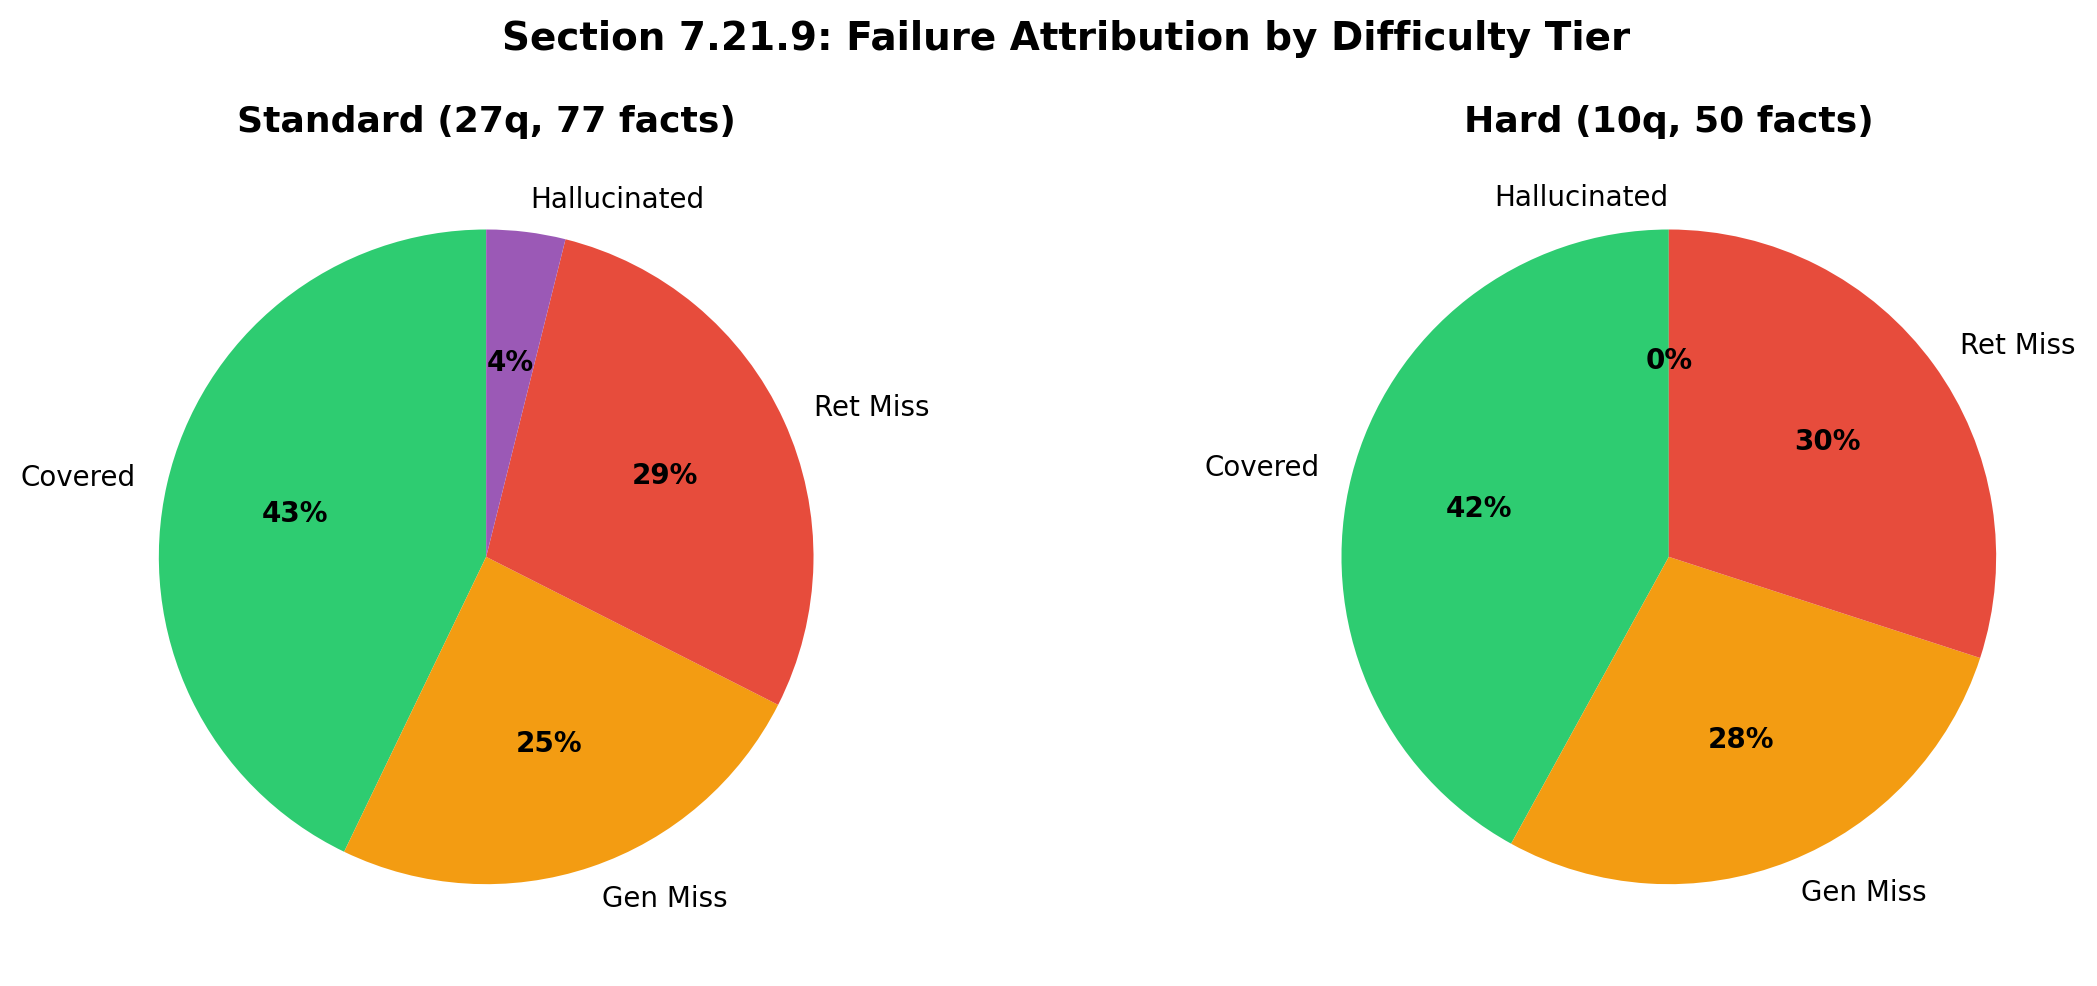
\includegraphics[width=0.85\linewidth]{docs/figures/chart18_failure_attribution_by_tier.png}
  \caption{Failure attribution by question difficulty tier. For standard questions, generation failures dominate. For hard multi-step questions, the bottleneck is fact volume (5--6 facts vs.\ 2--3), not cross-document synthesis per se.}
  \label{fig:failure_attribution}
\end{figure}

\textbf{Hard multi-step questions.} We created 10 hard questions requiring synthesis across 2--4 legal domains (e.g., security deposit violations as eviction defense, lead paint retaliation). Contrary to our hypothesis, hard question retrieval coverage (0.700) was slightly \emph{higher} than standard (0.675), and generation coverage given retrieval was also higher (0.714 vs.\ 0.654). The real bottleneck for hard questions is \textbf{fact volume}: with 5--6 key facts vs.\ 2--3 for standard questions, the LLM's tendency to omit secondary details (F1, F2) becomes more damaging.

\textbf{Confounding factors.} Three factors may inflate the observed failure rates. First, some generation ``failures'' (F1, F2) may reflect overly specific key-fact definitions rather than genuine LLM shortcomings---e.g., a key fact expecting the exact citation ``MGL c.186 s.15B'' scores as a miss even when the LLM correctly explains the rule without citing the statute number. The QA data audit (Section~\ref{sec:eval_framework}, 61 fixes applied) mitigated but did not eliminate this issue. Second, retrieval failures F4 (Program/Term Mismatch) and F5 (Statute Retrieval Miss) are primarily caused by the general-purpose embedding model (\texttt{all-MiniLM-L6-v2}), which was not trained on legal text and struggles to bridge vocabulary gaps between casual tenant queries and formal legal terminology. Third, F7 (Cross-Encoder Domain Mismatch) is an upstream artifact: the \texttt{ms-marco} reranker was trained on web search data and sometimes ranks conversational FAQ content above authoritative statute chunks. These confounds suggest that targeted component upgrades (legal-domain embeddings, legal cross-encoder) would reduce failure rates beyond what pipeline-level changes can achieve.

\subsection{Advanced Retriever Strategies}
\label{sec:advanced_retrievers}

Four additional retrieval strategies were evaluated on 27 stratified questions:

\begin{itemize}
    \item \textbf{Auto-merge:} Best retrieval coverage (0.727 vs.\ 0.675 baseline), with large gains on lead paint (+0.833) and retaliation (+0.200), but generation coverage dropped (0.589) due to context flooding---too many merged chunks overwhelm the LLM.
    \item \textbf{Hybrid + parent-child + rerank:} Best for rent\_increases (+0.333 vs.\ baseline).
    \item \textbf{Multi-query expansion:} Underperformed (1 improved, 5 regressed)---query variants may not have been sufficiently diverse.
    \item \textbf{Sentence window:} Weakest (1 improved, 10 regressed)---sentence-level embeddings were too short for legal question matching.
\end{itemize}

\subsection{Embedding Model Comparison}

We compared BGE-large-en-v1.5 (1024-dim) against the default all-MiniLM-L6-v2 (384-dim) on all 89 questions. The larger model performed slightly worse on all retrieval metrics (MRR $-$0.021, Recall@K $-$0.023, NDCG@K $-$0.028). This result is consistent with \citet{wiratunga2024cbrrag}, who found that \emph{domain-specific} embeddings (e.g., LegalBERT) outperform general-purpose ones for legal retrieval---but did not find that larger general-purpose models outperform smaller ones. Our comparison swapped one general-purpose model for another; neither was trained on legal text, so the larger embedding space (1024 vs.\ 384 dimensions) does not capture legal semantic distinctions like ``quiet enjoyment'' or ``tenancy at will.'' Additionally, the entire pipeline (chunking parameters, retrieval thresholds, top\_k tuning) was developed and optimized with MiniLM embeddings; swapping to BGE-large changes the similarity score distribution without re-tuning these parameters. For a 967-chunk corpus, 384 dimensions is already sufficient to distinguish chunks---the bottleneck is semantic understanding of legal terms, not vector space capacity.

\subsection{Challenges and Limitations}

\textbf{Cross-encoder domain mismatch (F7).} The ms-marco cross-encoder, trained on web search data, sometimes displaces formal legal statute chunks in favor of conversational FAQ content that scores higher on surface-level relevance. A legal-domain cross-encoder would likely improve statute retrieval.

\textbf{Evaluation metric limitations.} Binary faithfulness is coarse---a response that fabricates one statute reference scores the same as one that fabricates ten. Per-claim faithfulness scoring would provide finer granularity. Correctness is sensitive to judge identity (scores range from 0.321 to 0.750 for identical responses depending on the judge model).

\textbf{Fine-tuning format damage.} The Qwen3 fine-tuning failure highlights the fragility of chat template formatting in LoRA fine-tuning. Even corrected later training runs could not overcome damage from initial format-mismatched epochs.

\textbf{Corpus coverage.} Despite 249 documents, coverage gaps remain in areas like rent stabilization specifics, MRVP voucher details, and Housing Court procedural rules. The corpus is also a point-in-time snapshot that may become stale as laws change.

%----------------------------------------------------------------------
\section{Conclusion and Future Work}
\label{sec:conclusion}

We developed and iteratively evaluated a RAG-based legal question answering system for Massachusetts tenant law, demonstrating that retrieval augmentation dramatically improves LLM faithfulness (0.146 $\rightarrow$ 0.891) across all model families. Our systematic comparison of five retrieval strategies and four LLM families reveals that reranking provides the best balance of faithfulness and correctness, that Mistral Small 24B achieves comparable faithfulness to GPT-4o at 21$\times$ lower cost, and that even a 4B-parameter local model with RAG can rival cloud models on factual recall. Our failure taxonomy identifies generation-side failures as the primary bottleneck for standard legal queries, shifting attention from retrieval improvements to generation-aware solutions.

Future work should pursue: (1) retraining the Qwen3 fine-tuned model with corrected ChatML format data, (2) replacing the ms-marco cross-encoder with a legal-domain reranker to address failure mode F7, (3) implementing multi-pass generation to reduce statute citation dropout (F1) and remedy omission (F2), (4) adopting Summary-Augmented Chunking \citep{nllp2025reliable} to reduce document-level retrieval mismatch, and (5) expanding the corpus with Housing Court decisions and rent stabilization statutes to close remaining coverage gaps.

%----------------------------------------------------------------------

\begin{ack}
This work was completed as part of CS6180: Generative AI at Northeastern University, Spring 2026, taught by Prof.\ Ryan Rad. We thank the course staff for feedback on the evaluation methodology. All API costs for evaluation experiments were individually funded by the team members, En-Ping Su and Maxwell Berry. All data was scraped from publicly available government and legal aid websites. This system provides legal \emph{information}, not legal \emph{advice}.
\end{ack}

{\small

\bibliographystyle{plainnat}

\begin{thebibliography}{10}

\bibitem[Ajay~Mukund and Easwarakumar(2025)]{symmetry2025legal}
Ajay~Mukund~S and K.~S.~Easwarakumar.
\newblock Optimizing legal text summarization through dynamic retrieval-augmented generation and domain-specific adaptation.
\newblock \emph{Symmetry}, 17(5):633, 2025.

\bibitem[Es et~al.(2024)]{es2024ragas}
Shahul Es, Jithin James, Luis Espinosa-Anke, and Steven Schockaert.
\newblock {RAGAS}: Automated evaluation of retrieval augmented generation.
\newblock In \emph{Proceedings of EACL 2024 (System Demonstrations)}, 2024.

\bibitem[Gao et~al.(2024)]{gao2024ragsurvey}
Yunfan Gao, Yun Xiong, Xinyu Gao, Kangxiang Jia, Jinliu Pan, Yuxi Bi, Yi Dai, Jiawei Sun, Meng Wang, and Haofen Wang.
\newblock Retrieval-augmented generation for large language models: A survey.
\newblock \emph{arXiv preprint arXiv:2312.10997}, 2024.

\bibitem[Hindi et~al.(2025)]{rag_legal_survey_2025}
Mahd Hindi, Linda Mohammed, Ommama Maaz, and Abdulmalik Alwaraly.
\newblock Enhancing the precision and interpretability of retrieval-augmented generation ({RAG}) in legal technology: A survey.
\newblock \emph{IEEE Access}, 2025.

\bibitem[Kalra et~al.(2024)]{kalra2024hyparag}
Rishi Kalra, Zekun Wu, Ayesha Gulley, Airlie Hilliard, Xin Guan, Adriano Koshiyama, and Philip Treleaven.
\newblock {HyPA-RAG}: A hybrid parameter adaptive retrieval-augmented generation system for {AI} legal and policy applications.
\newblock In \emph{EMNLP 2024 CustomNLP4U Workshop}, 2024.

\bibitem[Li et~al.(2025)]{legaldc2025}
Yaocong Li, Qiang Lan, Leihan Zhang, and Le Zhang.
\newblock Legal-{DC}: Benchmarking retrieval-augmented generation for legal documents.
\newblock \emph{arXiv preprint arXiv:2603.11772}, 2025.

\bibitem[Magesh et~al.(2025)]{magesh2025hallucination}
Varun Magesh, Faiz Surani, Matthew Dahl, Mirac Suzgun, Christopher~D. Manning, and Daniel~E. Ho.
\newblock Hallucination-free? {Assessing} the reliability of leading {AI} legal research tools.
\newblock \emph{Journal of Empirical Legal Studies}, 22:216--242, 2025.

\bibitem[Pipitone and Alami(2024)]{legalbenchrag2024}
Nicholas Pipitone and Ghita~Houir Alami.
\newblock {LegalBench-RAG}: A benchmark for retrieval-augmented generation in the legal domain.
\newblock \emph{arXiv preprint arXiv:2408.10343}, 2024.

\bibitem[Reuter et~al.(2025)]{nllp2025reliable}
Markus Reuter, Tobias Lingenberg, R\={u}ta Liepi\c{n}a, Francesca Lagioia, Marco Lippi, Giovanni Sartor, Andrea Passerini, and Burcu Sayin.
\newblock Towards reliable retrieval in {RAG} systems for large legal datasets.
\newblock In \emph{Natural Legal Language Processing Workshop 2025 (EMNLP)}, 2025.

\bibitem[Wiratunga et~al.(2024)]{wiratunga2024cbrrag}
Nirmalie Wiratunga, Ramitha Abeyratne, Lasal Jayawardena, Kyle Martin, Stewart Massie, Ikechukwu Nkisi-Orji, Ruvan Weerasinghe, Anne Liret, and Bruno Fleisch.
\newblock {CBR-RAG}: Case-based reasoning for retrieval augmented generation in {LLMs} for legal question answering.
\newblock In \emph{ICCBR 2024}, 2024.

\end{thebibliography}
}

%%%%%%%%%%%%%%%%%%%%%%%%%%%%%%%%%%%%%%%%%%%%%%%%%%%%%%%%%%%%

\appendix

\section{System Architecture and Implementation Details}

The complete system is organized into the following modules:

\textbf{Data collection} (\texttt{src/scraping/}): Seven scrapers targeting mass.gov, boston.gov, BostonHousing.org, MassLegalHelp.org, and GBLS. Includes a browser-based fallback scraper for pages that block automated requests (403 errors). Shared utilities handle HTML fetching, cleaning, Markdown conversion, and citation extraction.

\textbf{Processing} (\texttt{src/processing/}): Recursive character splitter with Markdown-aware boundaries and content-type-specific handlers (FAQ, statute, generic). Post-processing corpus cleaner with 10+ filter stages. Sentence window chunker for alternative chunking experiments.

\textbf{RAG pipeline} (\texttt{src/rag/}): Core pipeline with ChromaDB vector store, 5 retriever implementations in a unified registry, structured prompt templates, and citation verification. Additional modules for multi-query expansion and hybrid parent-child retrieval.

\textbf{Evaluation} (\texttt{src/evaluation/}): Scorer with 13 configurations, LLM judge via Claude Sonnet 4, retrieval-aware correctness decomposition, multi-run averaging with parallel execution, automated QA data audit, and chart generation scripts.

\textbf{Frontend}: Next.js 16 (App Router) + React 19 chat interface with Tailwind CSS styling. Configuration sidebar for model selection (GPT-4o, Llama 3.3 70B, Mistral Small 24B), retriever strategy, top\_k parameter, and RAG toggle. Streaming responses via Server-Sent Events from the FastAPI backend (\texttt{api/server.py}).

\textbf{Fine-tuning} (\texttt{Fine-Tuneing/}): Data preparation script generating ChatML-format training data from golden QA, Reddit questions, and chunk-derived synthetic QA. Unsloth LoRA fine-tuning script for Qwen3 4B Instruct with early stopping.

%%%%%%%%%%%%%%%%%%%%%%%%%%%%%%%%%%%%%%%%%%%%%%%%%%%%%%%%%%%%

\newpage
\section*{NeurIPS Paper Checklist}

\begin{enumerate}

\item {\bf Claims}
    \item[] Question: Do the main claims made in the abstract and introduction accurately reflect the paper's contributions and scope?
    \item[] Answer: \answerYes{}
    \item[] Justification: The abstract and introduction state specific, quantified claims (faithfulness improvement from 0.146 to 0.891, 5 retrieval strategies, 4 model families, 8-mode failure taxonomy) that are directly supported by experimental results in Section~4.

\item {\bf Limitations}
    \item[] Question: Does the paper discuss the limitations of the work performed by the authors?
    \item[] Answer: \answerYes{}
    \item[] Justification: Section~4.9 discusses limitations including cross-encoder domain mismatch, evaluation metric coarseness, fine-tuning format damage, and corpus coverage gaps.

\item {\bf Theory assumptions and proofs}
    \item[] Question: For each theoretical result, does the paper provide the full set of assumptions and a complete (and correct) proof?
    \item[] Answer: \answerNA{}
    \item[] Justification: This paper is an empirical applied research project with no theoretical results or proofs.

    \item {\bf Experimental result reproducibility}
    \item[] Question: Does the paper fully disclose all the information needed to reproduce the main experimental results of the paper to the extent that it affects the main claims and/or conclusions of the paper (regardless of whether the code and data are provided or not)?
    \item[] Answer: \answerYes{}
    \item[] Justification: Section~3 provides full details on corpus construction, chunking parameters (800 tokens, 200 overlap), retriever configurations, model identifiers (OpenRouter format), evaluation metrics, judge model, and question set composition. Section~4 reports all hyperparameters for each experiment.

\item {\bf Open access to data and code}
    \item[] Question: Does the paper provide open access to the data and code, with sufficient instructions to faithfully reproduce the main experimental results, as described in supplemental material?
    \item[] Answer: \answerYes{}
    \item[] Justification: Code is provided via GitHub repository with README and requirements.txt. The corpus is constructed from publicly available government websites with scraping scripts included.

\item {\bf Experimental setting/details}
    \item[] Question: Does the paper specify all the training and test details (e.g., data splits, hyperparameters, how they were chosen, type of optimizer) necessary to understand the results?
    \item[] Answer: \answerYes{}
    \item[] Justification: Section~3.6 specifies fine-tuning details (LoRA rank=16, alpha=32, 3 epochs, 586 samples, Unsloth framework, RTX 5080). Section~3.5 specifies evaluation setup (89 questions, Claude Sonnet 4 judge, binary and per-fact metrics).

\item {\bf Experiment statistical significance}
    \item[] Question: Does the paper report error bars suitably and correctly defined or other appropriate information about the statistical significance of the experiments?
    \item[] Answer: \answerYes{}
    \item[] Justification: Section~4.7 reports multi-run averaging with standard deviation and 95\% confidence intervals from 3 parallel runs (e.g., faithfulness 0.891 $\pm$ 0.024, 95\% CI [0.865, 0.918]). The variance source is identified as LLM generation non-determinism.

\item {\bf Experiments compute resources}
    \item[] Question: For each experiment, does the paper provide sufficient information on the computer resources (type of compute workers, memory, time of execution) needed to reproduce the experiments?
    \item[] Answer: \answerYes{}
    \item[] Justification: Fine-tuning was performed on an RTX 5080 (~8 min). Local model inference used llama-server with GGUF F16 format. Cloud models were accessed via OpenRouter API. Evaluation used 3 cloud workers and 3 judge workers in parallel.

\item {\bf Code of ethics}
    \item[] Question: Does the research conducted in the paper conform, in every respect, with the NeurIPS Code of Ethics \url{https://neurips.cc/public/EthicsGuidelines}?
    \item[] Answer: \answerYes{}
    \item[] Justification: The system provides legal information (not advice), uses only publicly available government data, and includes appropriate disclaimers about its limitations.

\item {\bf Broader impacts}
    \item[] Question: Does the paper discuss both potential positive societal impacts and negative societal impacts of the work performed?
    \item[] Answer: \answerYes{}
    \item[] Justification: The introduction discusses the positive impact of improving access to legal information for renters. The paper explicitly distinguishes legal information from legal advice and notes hallucination risks (Section~4.9). The failure taxonomy (Section~4.8) characterizes specific risk modes.

\item {\bf Safeguards}
    \item[] Question: Does the paper describe safeguards that have been put in place for responsible release of data or models that have a high risk for misuse (e.g., pre-trained language models, image generators, or scraped datasets)?
    \item[] Answer: \answerNA{}
    \item[] Justification: The system uses existing LLMs via API and a small LoRA adapter trained on public government data. No high-risk models or datasets are released.

\item {\bf Licenses for existing assets}
    \item[] Question: Are the creators or original owners of assets (e.g., code, data, models), used in the paper, properly credited and are the license and terms of use explicitly mentioned and properly respected?
    \item[] Answer: \answerYes{}
    \item[] Justification: All data sources (mass.gov, boston.gov, MassLegalHelp.org, BostonHousing.org, GBLS) are publicly available government resources. Model providers (OpenAI, Meta, Mistral, Alibaba/Qwen, Anthropic) are credited. ChromaDB and HuggingFace models are cited.

\item {\bf New assets}
    \item[] Question: Are new assets introduced in the paper well documented and is the documentation provided alongside the assets?
    \item[] Answer: \answerYes{}
    \item[] Justification: The curated evaluation dataset (89 questions with key facts and source chunk references) and the failure taxonomy are documented in the paper and code repository.

\item {\bf Crowdsourcing and research with human subjects}
    \item[] Question: For crowdsourcing experiments and research with human subjects, does the paper include the full text of instructions given to participants and screenshots, if applicable, as well as details about compensation (if any)?
    \item[] Answer: \answerNA{}
    \item[] Justification: This project does not involve crowdsourcing or human subjects research.

\item {\bf Institutional review board (IRB) approvals or equivalent for research with human subjects}
    \item[] Question: Does the paper describe potential risks incurred by study participants, whether such risks were disclosed to the subjects, and whether Institutional Review Board (IRB) approvals (or an equivalent approval/review based on the requirements of your country or institution) were obtained?
    \item[] Answer: \answerNA{}
    \item[] Justification: This project does not involve human subjects research.

\item {\bf Declaration of LLM usage}
    \item[] Question: Does the paper describe the usage of LLMs if it is an important, original, or non-standard component of the core methods in this research? Note that if the LLM is used only for writing, editing, or formatting purposes and does \emph{not} impact the core methodology, scientific rigor, or originality of the research, declaration is not required.
    \item[] Answer: \answerYes{}
    \item[] Justification: LLMs are the core component of this research---used as both the response generators (GPT-4o, Llama 3.3 70B, Mistral Small 24B, Qwen3 4B) and the evaluation judge (Claude Sonnet 4). All model identifiers, API providers, and evaluation prompts are fully specified.

\end{enumerate}



\end{document}
